\documentclass[11pt, a4paper, spanish]{article}

%%%%%%%%%% COMIENZO DEL PREAMBULO %%%%%%%%%%

%Info sobre este documento
\author{Martin Cammi}
\title{Trabajo Pr'actico de Ingenier'ia del software I}

%\usepackage{infostyle}                                                  % provee un look & feel similar a un documento Word
\usepackage[top=2.5cm, bottom=2.5cm, left=2.5cm, right=2.5cm]{geometry}  % m\'argenes
\usepackage[ansinew]{inputenc}                                           % permite que los acentos del estilo \'a\'e\'i\'o\'u salgan joya
\usepackage[spanish, activeacute]{babel}                                 % idioma espa\~{n}ol, acentos f\'aciles y deletreo de palabras
\usepackage{indentfirst}                                                 % permite indentar un parrafo a mano
\usepackage{caratula}                                                    % incluye caratula est\'andar
\usepackage{graphicx}                                                    % permite insertar gr\'aficos
\usepackage{color}                                                       % permite el uso de colores en el documento
\usepackage[pdfcreator={TexLive!, LaTeX2e con TeXnicCenter y la inteligencia de Jonathan ;-)},
			pdfauthor={Grupo 1"},
			pdftitle={Ingenieria del Software - Trabajo practico: sistema de software CentralMarket},
			pdfsubject={Trabajo Practico de Modelado de dominio},
			pdfkeywords={Contenidos, proveedor, bajo demanda},
			pdfstartview=FitH,            % Fits the width of the page to the window
			bookmarksnumbered,            % los bookmarks numerados se ven mejor...
			colorlinks,                   % links con bellos colores
			linkcolor=magenta]            % permite cambiar el color de los links
			{hyperref}                    % Permite jugar con algunas cosas que aparecer\'an en el PDF final
\usepackage{hyperref}


%\selectlanguage{spanish}

\linespread{1.3}                    % interlineado equivalente al 1.5 l\'ineas de Word...
\pagestyle{myheadings}              %encabezado personalizable con \markboth{}{}
\markboth{}{Trabajo Modelado de Objetivos. (Abreg\'u, Cammi, De Sousa, M\'endez, Raffo) }
\headsep = 30pt                     % separaci\'on entre encabezado y comienzo del p\'arrafo

%\addtolength{\oddsidemargin}{-2cm}	% configuracion IDEAL!!!
%\addtolength{\textwidth}{4cm}
%\addtolength{\textheight}{2cm}

% macro 'todo' para To-Do's
\def\todo#1{\textcolor{red}{#1}}

% Macro 'borde' para un texto con borde
\newsavebox{\fmbox}
\newenvironment{borde}[1]
{\begin{lrbox}{\fmbox}\begin{minipage}{#1}}
{\end{minipage}\end{lrbox}\fbox{\usebox{\fmbox}}\\[10pt]}

%%%%%%%%%% FIN DEL PREAMBULO %%%%%%%%%%

\begin{document}

\materia{Ingenier\'ia de Software I}
\submateria{Primer Cuatrimestre de 2012}
\titulo{Reentrega \\Trabajo pr\'actico 2}
\subtitulo{Modelos de comportamiento del sistema de software para CentralMarket}
\grupo{Grupo 1}

\integrante{Abreg\'u, Angel}{082/09}{angelj\_a@hotmail.com}
\integrante{Cammi, Mart\'in}{676/02}{martincammi@gmail.com}
\integrante{De Sousa, Mariano}{389/08}{marian\_sabianaa@hotmail.com}
\integrante{M\'endez, Gonz\'alo}{843/04}{gemm83@hotmail.com}
\integrante{Raffo, Diego}{423/08}{enanodr@hotmail.com}


\maketitle

\thispagestyle{empty}

\tableofcontents

\newpage

% Conviene poner las secciones como diferentes archivos,
% sobre todo cuando se trabaja en equipo.
% Es m\'as f\'acil para sincronizar mediante control de versiones.
%\input{Introducci\'on}


% BEGIN Ejemplos de uso

	%\section{Una secci\'on}
	%\label{sec:unaSeccion}
	%Hola! Soy una Secci\'on
	%	\subsection{Una subsecci\'on}
	%		Y yo soy una subsecci\'on!!!
	%		\subsubsection{Una subsubsecci\'on}
	%			Y yo soy una sub-subsecci\'on!!!
	%			\paragraph{Un p\'arrafo\\}
	%				Y yo soy un p\'arrafo, porque no hay mas sub-sub-sub-subsecciones!!!

	%\section{Otra secci\'on}
	%	Como pudimos ver en la secci\'on \ref{sec:unaSeccion}, esto es una demo de una referencia a una secci\'on.
	
	%	Tambi\'en podemos hacer referencia a la p\'agina de la secci\'on:\\[10pt]
	
		% Ejemplo de uso de un borde (falta pulir para que no tire un warning!)
	%	\begin{borde}{0.98\textwidth}
	%		En la p\'agina \pageref{sec:unaSeccion}, hay una secci\'on pilla...
	%	\end{borde}

% END Ejemplos de uso


\section{Correcciones}
\label{sec:Correcciones}

\subsection{Puntos a corregir}

	A continuaci�n listamos los puntos de correci�n del Trabajo pr�ctico 2:

\begin{itemize}	
	
	\item{ \emph{Aclaraci\'on sobre las cuentas}: Aclarar que el resto de las cuentas (salvo la del usuario) ser�n creadas previamente por el administrador del sistema. }
	\item{ \emph{Amigo vs Usuario}: Justificar mejor lo referente a esta interacci\'on Amigo-Usuario o cambiar el dise�o. }
	\item{ \emph{Contenido Calificado}: Corregir Contenido Calificado y Contenido Recomendado, ambas podrian ser clases en si mismas, ajustar el OCL de forma adecuada. }
	\item{ \emph{Modelo de FSM}: Modelar con FSM la interacci�n entre los diversos dispositivos de un mismo usuario. }\\

	Prodeceremos entonces a enumerar las correciones al Tp2, destacando en \textbf{negrita} los cambios que sean peque\~{n}os.

\end{itemize}

\newpage

\section{Aclaraci�n sobre las cuentas}

	En el modelado a continuaci\'on asumiremos que todos los actores que interactuen con el sistema \textbf{(salvo el usuario, el cual deber� crearla el mismo)} ya tienen creada una cuenta previa para poder loguearse y realizar sus acciones.

\section{Amigo vs Usuario}


Se decidi� mantener el rol de \emph{Amigo} en los casos de uso ya que el pr\'estamo de contenido s\'olo tiene sentido entre personas que se conozcan entre s\'i y posean una relaci\'on de amistad. \\
Un usuario hasta no tener al menos un amigo, no puede realizar ning\'un pr\'estamo.\\

El sistema permite la creaci\'on de nuevas amistades, as\'i como la terminaci\'on de estas. Siempre que la cantidad de amigos de un usuario sea mayor estricto que cero, \'el podr\'a acceder a las funcionalidades de los pr\'estamos.\\

No es necesario que el usuario conozca esta diferencia de roles alcanza con que el sistema habilite o inhabilite la funcionalidad de pr\'estamos dependiendo de la cantidad de amigos asociados a un usuario.\\

\section{Contenido Calificado}

	\begin{center}
		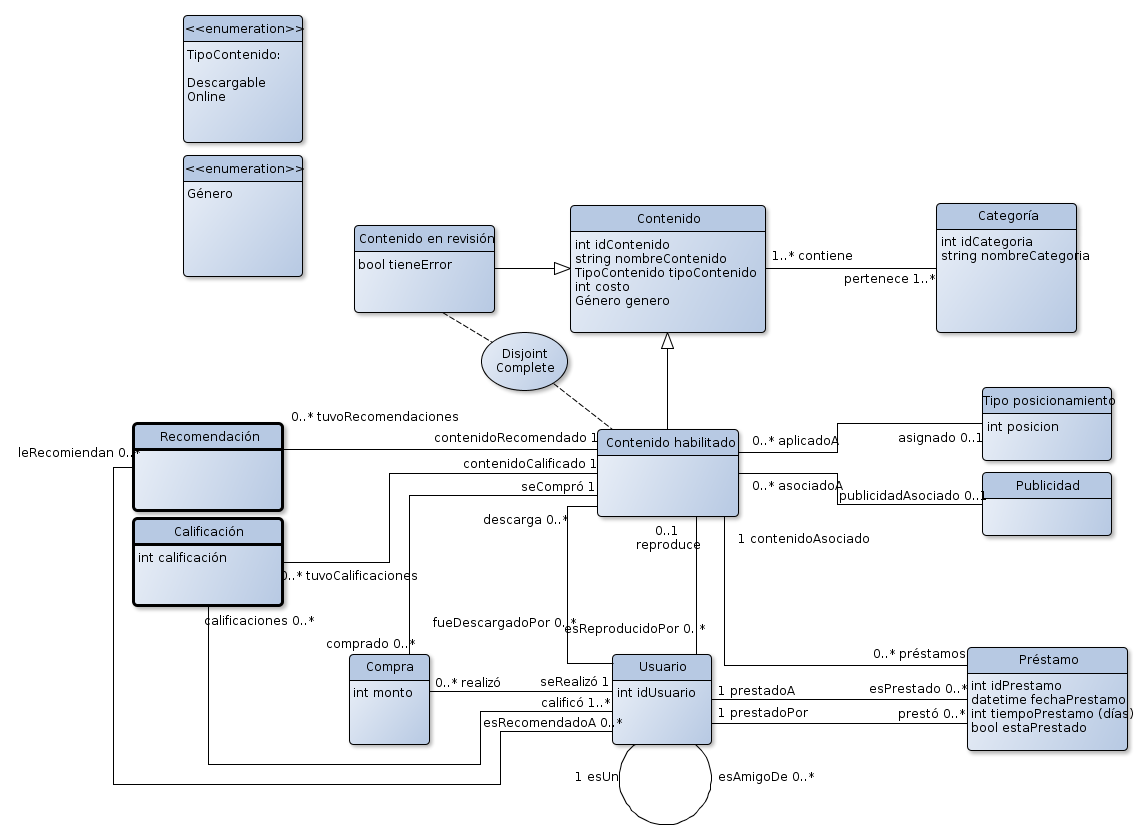
\includegraphics[scale=0.36]{Diagramas/09-ModeloConceptualMC.png}
	\end{center}
	
	\noindent{En negrita figuran las clases modificadas.}\\

	Se cambi� la clase \emph{Contenido Calificado} que heredaba de \emph{Contenido habilitado} por \emph{Calificaci�n} que se relaciona con Contenido habilitado.\\

	Se cambi� la clase \emph{Contenido Recomendado} que heredaba de \emph{Contenido habilitado} por \emph{Recomendaci�n} que se relaciona con Contenido habilitado.

\subsection{Cambios en el OCL}

	La modificaci\'on de clases anterior genera los siguientes cambios en el OCL:\\

\noindent{\textbf{Context Usuario}}\\
El usuario tiene contenido recomendado sii calific\'o al menos un contenido.\\
\noindent{\textbf{inv:} self.calificaciones$\rightarrow$isEmpty() $\Longleftrightarrow$ self.leRecomiendan$\rightarrow$isEmpty()}\\

\noindent{El usuario s\'olo calific\'o contenido que compr\'o (para todo contenido calificado, existe alguna compra hecha con ese contenido)}\\
\noindent{\textbf{inv:} self.calificaciones$\rightarrow$notEmpty() $\Longrightarrow$ self.realizo$\rightarrow$notEmpty() $\wedge$\\
self.calificaciones$\rightarrow$collect(contenidoCalificado)$\rightarrow$\\forAll( u $\mid$ self.realizo$\rightarrow$exists( c $\mid$ c.seCompro.idContenido $==$ u.idContenido))\\

\noindent{La cantidad de contenidos recomendados a un usuario es igual a cero (si nunca calific\'o) o diez (cuando ya calific\'o)}\\
\noindent{\textbf{inv:} ( self.calificaciones$\rightarrow$isEmpty() $\Longrightarrow$ self.leRecomiendan$\rightarrow$isEmpty() ) $\wedge$\\
( self.calificaciones$\rightarrow$notEmpty() $\Longrightarrow$ ( self.leRecomiendan$\rightarrow$size() $==$ 10 ) )\\

\noindent{No se recomienda contenido ya comprado ni contenido obtenido de pr\'estamos.}\\
\noindent{\textbf{inv:} self.leRecomiendan$\rightarrow$collect(contenidoRecomendado)$\rightarrow$forall(c $\mid$ c.comprado$\rightarrow$notEmpty() $\Longrightarrow$ c.comprado$\rightarrow$forall(c2 $\mid$ c2.seRealiz\'o.idUsuario $\ne$ self.seRealiz\'o.idUsuario))\\
\begin{center} \line(1,0){450} \end{center}

\noindent{\textbf{Context Calificaci\'on}}\\
Las calificaciones son de 0 a 10.\\
\noindent {\textbf{inv:} 0 $\leq$ self.calificaci\'on $\wedge$ self.calificaci\'on $\leq$ 10}


\newpage

\section{Modelo de FSM}

	A continuaci\'on modelaremos la interacci�n de los diversos dispositivos de una sola cuenta de usuario para la reproducci�n de contenido.

	\begin{center}
		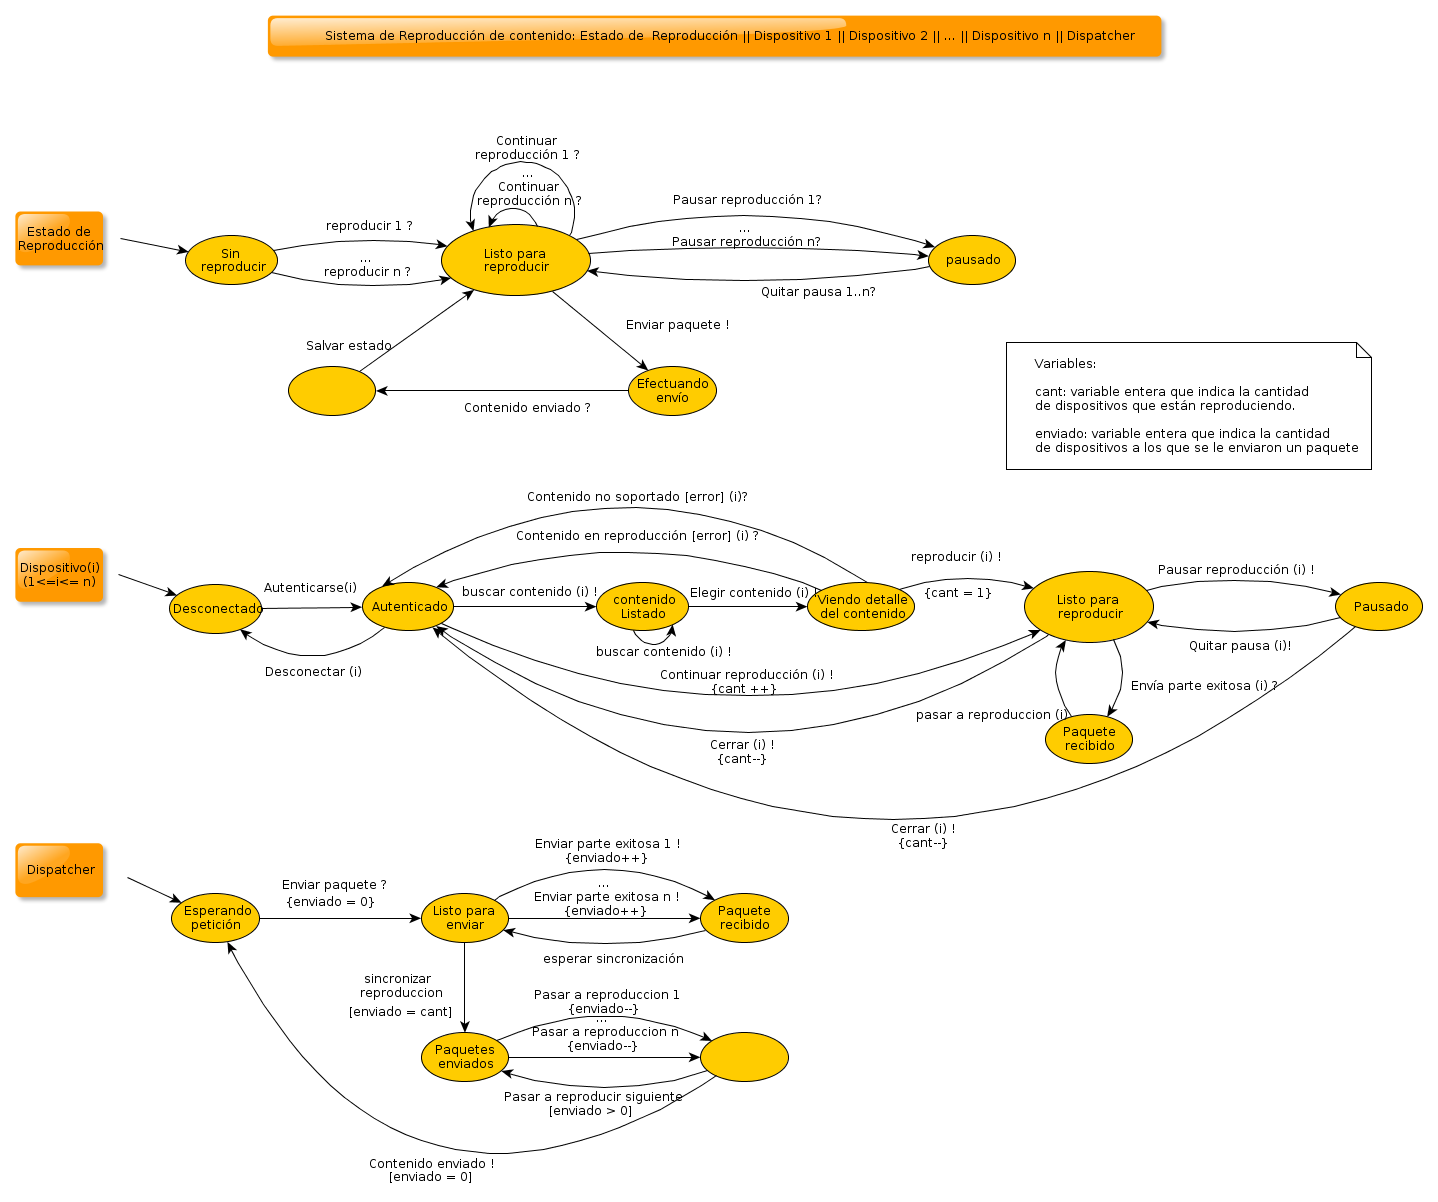
\includegraphics[scale=0.36]{Diagramas/FSM-ReproduccionContenido.png}
	\end{center}

Cosas que se pueden apreciar en el modelo:

\begin{itemize}
	
	\item{ S\'olamente se puede estar reproduciendo un s\'olo contenido para los diversos dispositivos de un usuario. } 
	\item{ Todos los dispositivos pueden estar reproduciendo contenido al mismo tiempo, pero \'este debe ser siempre el mismo (para la misma cuenta de usuario).} 
	\item{ Si un contenido en reproducci\'on est� siendo visto por varios dispositivos y uno de ellos pausa la reproducci\'on, el resto tambi\'en ser\'a pausado.}
	\item{ Se guarda el estado del \'ultimo paquete enviado exitosamente.}
	\item{ El \emph{Estado inicial} es para cuando no se ha comenzado a reproducir ning\'un contenido. El estado \emph{Sin reproducir (con estado)} indica que es posible continuar con la reproducci\'on de un contenido a\'un cuando todos los dispositivos se hayan desconectado. Adem\'as muestra que se puede elegir un nuevo contenido a reproducir si y s\'olo si todos los dispositivos cerraron.}

\end{itemize}

\newpage

\end{document}
